\subsection{问题2、3}
问题2与问题3的性质相同,均属于使用扫描得到的数据重建样品的吸收率分布(即形状),故二者可合并解决。

\subsubsection{数学原理:反投影}
本题要解决的问题实际为逆 Radon 变换,这个问题最早由数学家Johann Radon在1917年提出\cite{radon1986}。我们首先进行理论上的推导。

对于二维密度函数 $\mu(x, y)$,将其进行二维Fourier变换后所得的函数记为 $F(u, v)$,根据Fourier逆变换公式可以得到

\begin{equation}
	\mu(x, y) = \iint F(u, v) \mathrm e^{2\pi i(ux + vy)} \diff u \diff v
	\label{equ:2_inv_fourier}
\end{equation}

将空域变换为极坐标形式 $u = \rho\cos\theta, v = \rho\sin\theta$ 后可得

\begin{equation}
	\begin{aligned}
	\mu(x, y) &= \int_0^\infty\int_0^{2\pi} F(\rho, \theta) \mathrm e^{2\pi i \rho R} \rho\diff \theta \diff \rho \\
			&= \int_0^\infty\int_0^{\pi} F(\rho, \theta) \mathrm e^{2\pi i \rho R} \rho\diff \theta \diff \rho
			 +\int_{-\infty}^0\int_0^{\pi} F(-\rho, \theta + \pi) \mathrm e^{2\pi i \rho R} \rho\diff \theta \diff \rho
	\end{aligned}
	\label{equ:2_polar_inv_fourier}
\end{equation}

其中 $R = x\cos\theta + y\sin\theta$。由于$\mu(x, y)$为实值函数,其二维Fourier变换满足$F(\rho, \theta) = F(-\rho, \theta + \pi)$,因此

\begin{equation}
	\begin{aligned}
		\mu(x, y) &= \int_{-\infty}^\infty\int_0^{\pi} F(\rho, \theta) |\rho| \mathrm e^{2\pi i \rho R} \diff \theta \diff \rho \\
	\end{aligned}
	\label{equ:2_polar_inv_fourier2}
\end{equation}

利用Fourier中心切片定理\pagescite[][70-72]{kang2014},

\begin{equation}
	F(\rho, \theta) = \mathcal F_1\{ g_\theta(R) \}
	\label{equ:2_fourier_center_slicing}
\end{equation}

将公式\ref{equ:2_fourier_center_slicing}代入公式\ref{equ:2_polar_inv_fourier2}后可得

\begin{equation}
	\mu(x, y) = \int_0^{\pi} \mathcal F_1^{-1} \{ \mathcal F_1\{ g_\theta(R) \}\cdot |\rho| \} \diff \theta
	          = \int_0^\pi \hat g_\theta(R) \diff \theta
	\label{equ:2_fourier_conv}
\end{equation}

我们令 $\hat g_\theta(R) = \mathcal F_1^{-1} \{ \mathcal F_1\{ g_\theta(R) \}\cdot |\rho| \} = g_\theta(R) \ast \mathcal F^{-1}_1 \{ |\rho| \}$。注意到公式$\ref{equ:2_fourier_conv}$中右侧积分的意义相当于将$\hat g_\theta$作为吸收强度做直接反投影,因此我们得到了一个能较为精确还原出原始信息的算法。

推导中的$|\rho|$相当于一个滤波函数,我们所做的相当于利用其对$\mathcal F_1\{ g_\theta(R) \}$进行滤波后再变换回频域进行直接反投影。由于利用$g_\theta$做直接反投影和利用$\hat g_\theta$做直接反投影相差了一个与 $\mathcal F_1^{-1}\{ |\rho| \}$的卷积,原先的方法会造成如图像模糊等诸多问题。

\subsubsection{初步实现:直接反投影}
在本题的具体处理上,需要对180个方向分别进行反投影。对于每一个转动角度$\theta$下$xoy$系中的任意一点$P$,进行以下的处理:
\begin{enumerate}
  \item 寻找投影坐标:设待测点$P$在$xoy$坐标系中的坐标为$(x_p,y_p)$,在$XOY$坐标系的$OX$轴上的投影值为$R$。此时$OX$轴在$xoy$系中的直线方程为$y\cos\theta=x\sin\theta$,过P向其作垂线,方程为$(y-y_p)\sin\theta+(x-x_p)\cos\theta=0$,垂足即为$R$。联立方程即可解得$R_x=x_p\cos\theta+y_p\sin\theta$。
  \item 获取投影值:由于投影坐标一般不会落在接收器对应的坐标点上,故需要对接收器值进行插值。我们选取离坐标最近的两个接收器值进行线性插值,作为该点在此角度下的吸收值。
  \item 累加吸收值:将上一部中得到的吸收值加到该点原有的值上
\end{enumerate}

事实上,除了这种“像素驱动”(即,从点出发寻找线上坐标)的反投影方法外,还有“射线驱动”法,即每次从射线上一点作垂线,在射线上等距步进,每次前进一步就将采样值分配到相邻像素中。之所以没有采用这种方法,主要原因是求解射线与坐标系的小格相交问题比较困难,同时这种方法包含二维的插值,需要更大的运算量。

当所有转动角度均遍历过后,直接反投影过程即完成。尝试用本法反投影恢复题中附件所给数据的几何信息,得到的图形(图\ref{fig:2_direct:2})较为模糊,轮廓不清;椭圆周围有较广的晕影,几乎遮盖了小圆的部分。尝试恢复附件(3)时,出现了同样的问题(图\ref{fig:2_direct:3});对于附件(5),直接反投影的方法得到的途中充满了“伪影”,除大致轮廓外几乎没有有用的信息(图\ref{fig:2_direct:5})。

\begin{figure}[htbp]
  \centering

  \begin{subfigure}[b]{0.3\textwidth}
    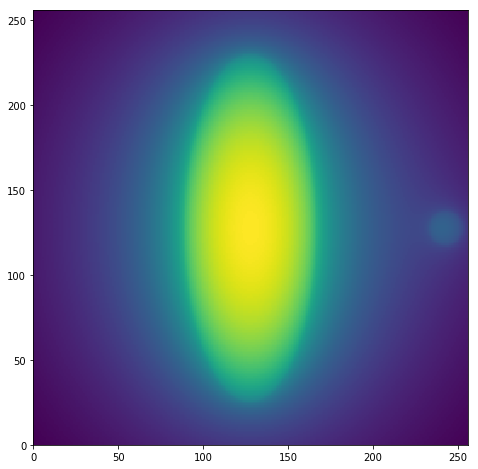
\includegraphics[width=\linewidth]{2_direct_2.png}
    \caption{附件(2)}
    \label{fig:2_direct:2}
  \end{subfigure}%
  \hfill
  \begin{subfigure}[b]{0.3\textwidth}
    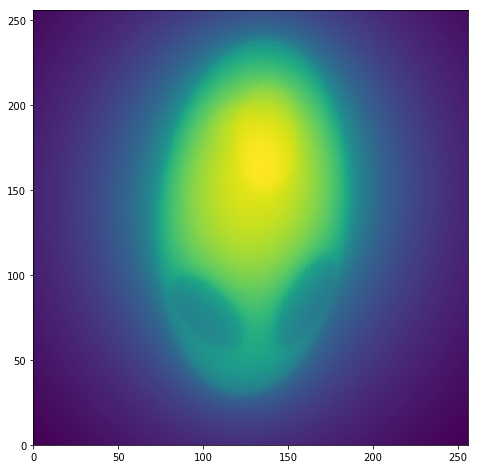
\includegraphics[width=\linewidth]{2_direct_3.png}
    \caption{附件(3)}
    \label{fig:2_direct:3}
  \end{subfigure}%
  \hfill
  \begin{subfigure}[b]{0.3\textwidth}
    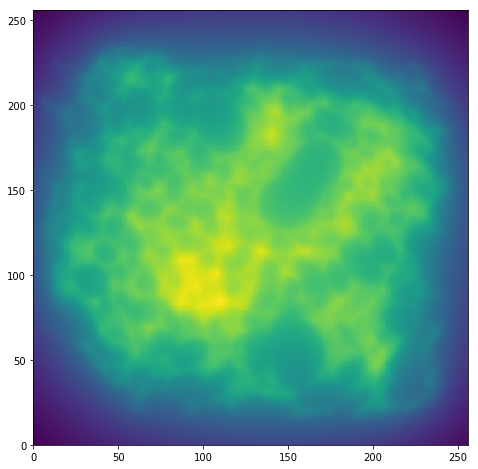
\includegraphics[width=\linewidth]{2_direct_5.png}
    \caption{附件(5)}
    \label{fig:2_direct:5}
  \end{subfigure}

  \caption{直接反投影恢复出的介质}
  \label{fig:2_direct}
\end{figure}

\subsubsection{改进:滤波反投影}
由于直接反投影法的缺陷,根据公式\ref{equ:2_fourier_conv},我们可以通过在进行反投影前对投影数据进行滤波处理以提高结果的准确度。对于每一个旋转角度$\theta$,在遍历像素前先进行以下处理:
\begin{enumerate}
  \item DFT:将接收器坐标点对应的吸收值进行离散 Fourier 变换
  \item 滤波:在上一步所得的频域结果上乘给定的滤波函数
  \item IDFT:将上一部所得的结果进行逆离散 Fourier 变换,并去除所有结果的虚部,只保留实部作为新的吸收值
\end{enumerate}

关于滤波器的选择,许多文献均有比较详细的介绍\cite{gao2010}\pagescite[][96-97]{gu2012}\pagescite[][80-82]{kang2014}。作为测试,我们尝试了R-L滤波器、S-L滤波器、Hanning滤波器等多种不同的函数。由于R-L滤波函数在工业界被广泛使用、原理与实现比较简单、与其他滤波器效果也没有明显劣势,我们将其作为最终的选择。在R-L滤波器算法的实现部分,我们参考了 Matlab 中 \texttt{iradon} 函数的实现\pagescite[][70-76]{kak2001}。

图\ref{fig:2_filter}为对三个附件分别进行滤波反投影得到的图像。从直观上图像的清晰度、辨识度都有了极大的提升。图\ref{fig:2_direct:2}与附件(2)给出的模型吻合度高,完整地恢复出了圆、椭圆的内部,吸收率分布也很均匀。附件(3)(图\ref{fig:2_direct:3})的介质主体形状为一个放置不正的椭圆,内有五个近似椭圆形的吸收率不同的区域:下部两个区域吸收率很低,中部的一个接近介质其他部分,上部的两个吸收率较高,并有重叠(重叠部分为两者吸收率之和)。附件(5)(图\ref{fig:2_direct:5})是一种多孔的稀疏介质,介质的吸收率分布并不均匀。

\begin{figure}[htbp]
  \centering

  \begin{subfigure}[b]{0.3\textwidth}
    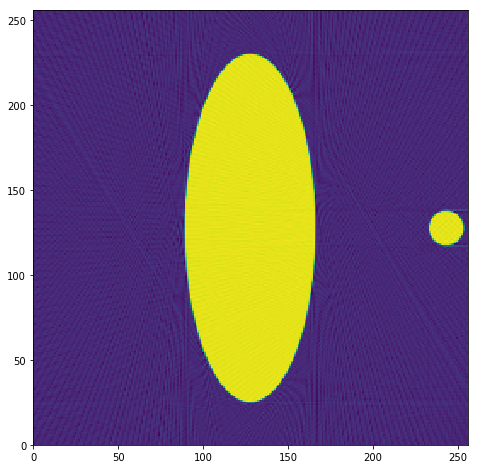
\includegraphics[width=\linewidth]{2_filter_2.png}
    \caption{附件(2)}
    \label{fig:2_filter:2}
  \end{subfigure}%
  \hfill
  \begin{subfigure}[b]{0.3\textwidth}
    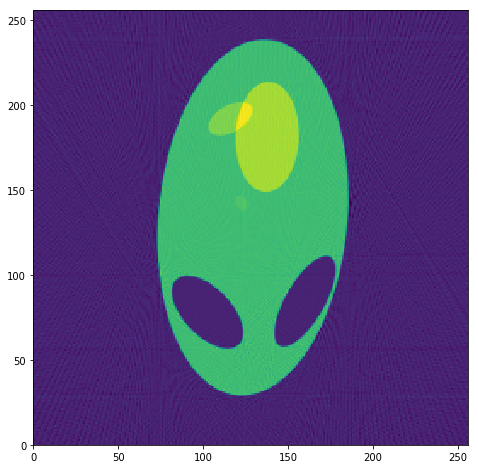
\includegraphics[width=\linewidth]{2_filter_3.png}
    \caption{附件(3)}
    \label{fig:2_filter:3}
  \end{subfigure}%
  \hfill
  \begin{subfigure}[b]{0.3\textwidth}
    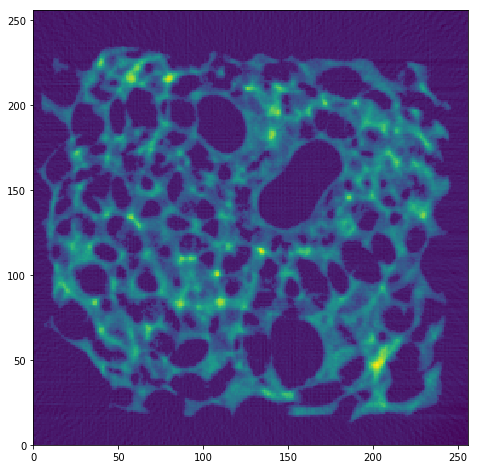
\includegraphics[width=\linewidth]{2_filter_5.png}
    \caption{附件(5)}
    \label{fig:2_filter:5}
  \end{subfigure}

  \caption{滤波反投影恢复出的介质}
  \label{fig:2_filter}
\end{figure}

\subsubsection{最终:计算吸收率}

最终每点的吸收率需要对数据进行归一化:计算重建附件(2)得到的圆与椭圆内部的吸收率平均值(再除$1.00$),此即为在我们恢复得到的一点的数值与题目给出的吸收率的比例因子;根据比例因子即可将样例(2)与(3)的每点数值转化为对应的吸收率。所有的吸收率数据已按照题目要求在附件中给出。

由于题目所给的10个位置在进行坐标转换后并非落在$256 \times 256$坐标的整数点上,故我们需要对每个点的吸收率进行重新计算,以确保数据的准确。计算方法与上面完全是相同的,仅仅将每次遍历的点变为给定的10个。最后我们得到了附录中的表\ref{table:absort_rate}中的结果。由于不可避免的噪声影响与算法的局限性,计算出部分点的吸收值为负;为了符合真实情况,我们将负数结果统一置为$0$。同时我们也将这10个点对应绘制在了图\ref{fig:2_dots}上,以供参考。

\begin{figure}[htbp]
  \centering

  \begin{subfigure}[b]{0.3\textwidth}
    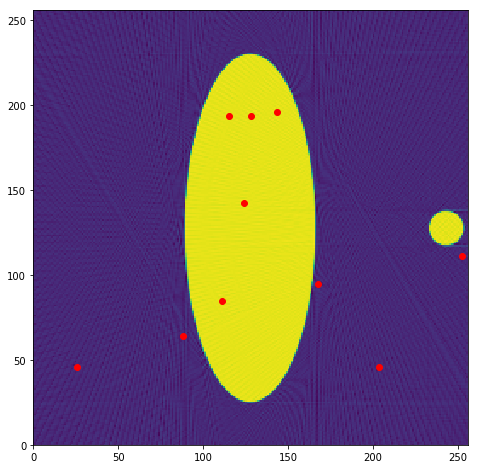
\includegraphics[width=\linewidth]{2_dots_2.png}
    \caption{附件(2)}
    \label{fig:2_dots:2}
  \end{subfigure}%
  \hfill
  \begin{subfigure}[b]{0.3\textwidth}
    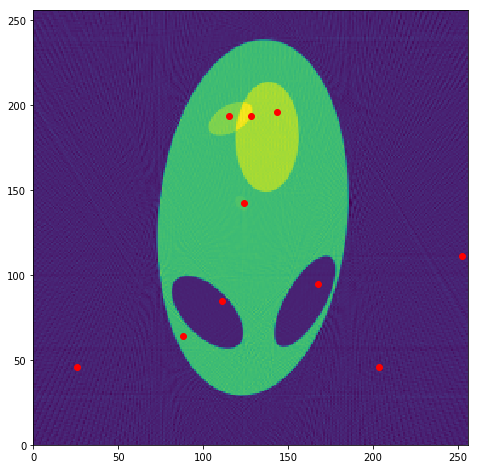
\includegraphics[width=\linewidth]{2_dots_3.png}
    \caption{附件(3)}
    \label{fig:2_dots:3}
  \end{subfigure}%
  \hfill
  \begin{subfigure}[b]{0.3\textwidth}
    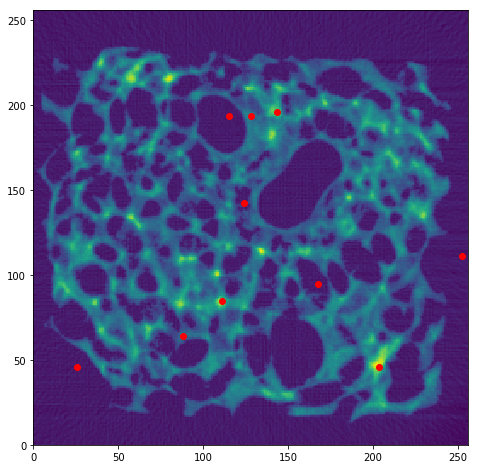
\includegraphics[width=\linewidth]{2_dots_5.png}
    \caption{附件(5)}
    \label{fig:2_dots:5}
  \end{subfigure}

  \caption{恢复出的图像上给定的坐标点}
  \label{fig:2_dots}
\end{figure} 